% !TEX root = main.tex

\subsection{Fit Knowledge Base}

\begin{figure}[!]
    \centering
    % \vspace{-0.2em}
    \begin{subfigure}[]{0.24\textwidth}
        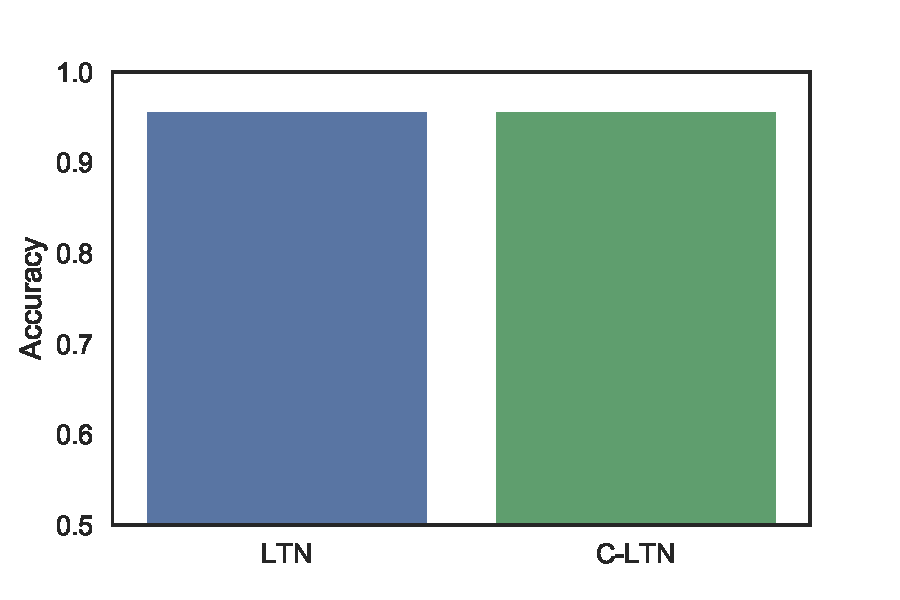
\includegraphics[width=\textwidth]{img/bar1.pdf}
        \caption{Best Accuracy on Group1}
        \label{fig:fitting-best-accuracy-1}
        %\vspace{-0.3em}
    \end{subfigure}~~~~
    \begin{subfigure}[]{0.24\textwidth}
        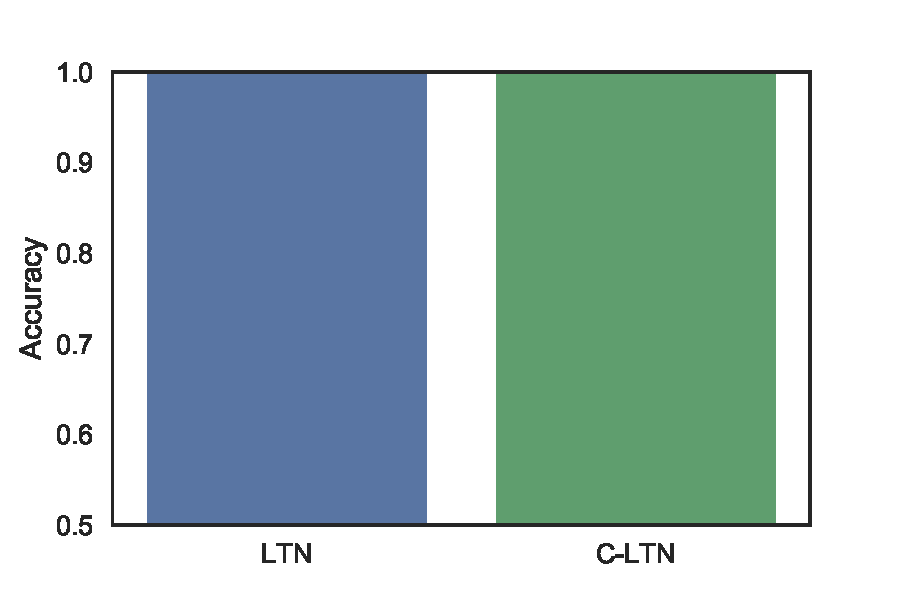
\includegraphics[width=\textwidth]{img/bar2.pdf}
        \caption{Best Accuracy on Group2}
        \label{fig:fitting-best-accuracy-2}
        %\vspace{-0.8em}
    \end{subfigure}

    \begin{subfigure}[]{0.24\textwidth}
        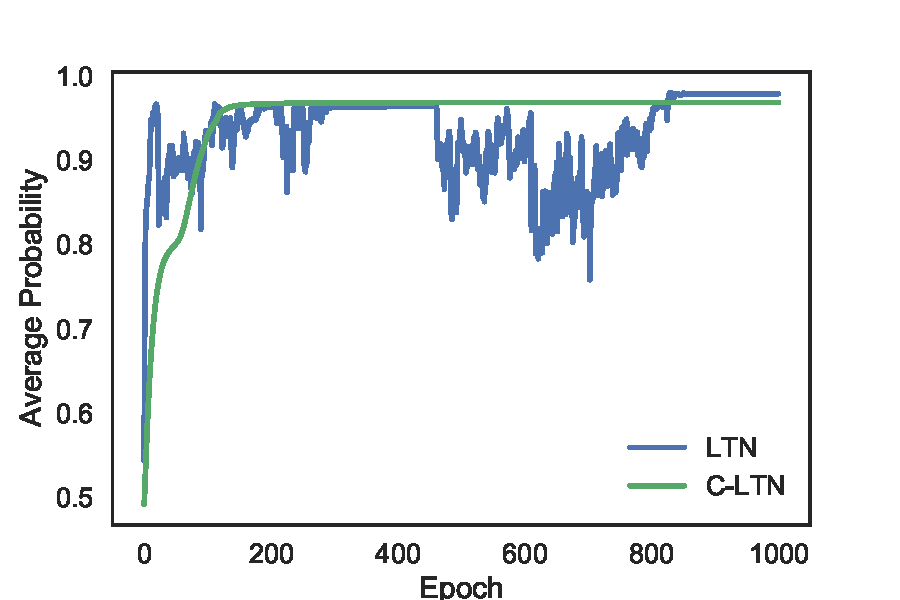
\includegraphics[width=\textwidth]{img/curve1.pdf}
        \caption{Probability w.r.t. Epoch}
        \label{fig:fitting-prob-epoch}
        %\vspace{-0.3em}
    \end{subfigure}
    \caption{Fitting Observed Facts.}
    \label{fig:fitting}
    % \vspace{-1.2em}
\end{figure}

In this experiment, we only use the oberserved facts, which is $K_{exp1} = K^{SFC}_{a \dots h} \cup K^{SF}_{i\dots n}$.

As there is no rules in this part, so we only compare the result of LTN and C-LTN.
Figure \ref{fig:fitting} shows the result of this experiment, where Figure \ref{fig:fitting-prob-epoch} is the probability change with respect to the training epoch, Figure \ref{fig:fitting-best-accuracy-1} shows the accuracy on the first group and Figure \ref{fig:fitting-best-accuracy-2} is that of the second group.

From the Figure \ref{fig:fitting}, it's clear that both LTN and C-LTN fit the observed data very well. The reason why the accuracy on first group is not $100\%$ is that there exists a contradictory pair: $S(g)$ and $\neg S(g)$. So it's not possible to make both of them $100\%$ true.

Another interesting phenomenon is that the curve of C-LTN is much more smooth than that of LTN, indicating that the training process of C-LTN is more stable and therefore easier to converge to a good result.

Here we also shows the fitting result for each predicate on two groups in Table \ref{table:fitting-group-1} and Table \ref{table:fitting-group-2}. And it's clear that we have a good fitting to the obseverd data.

\begin{table}[]
\centering
\begin{tabular}{c|c|c|cccccccc}
\toprule
\multirow{2}{*}{} & \multirow{2}{*}{S} & \multirow{2}{*}{C} & \multicolumn{8}{c}{F}                                 \\ \cmidrule{4-11}
                  &                    &                    & a    & b    & c    & d    & e    & f    & g    & h    \\ \midrule
a                 & 1.00               & 1.00               & 1.00 & 1.00 & 0.00 & 0.00 & 1.00 & 1.00 & 1.00 & 0.00 \\
b                 & 0.00               & 0.00               & 1.00 & 0.11 & 1.00 & 0.00 & 0.00 & 0.00 & 0.00 & 0.00 \\
c                 & 0.00               & 0.00               & 0.00 & 1.00 & 0.01 & 1.00 & 0.00 & 0.00 & 0.00 & 0.00 \\
d                 & 0.00               & 0.00               & 0.00 & 0.00 & 1.00 & 0.00 & 0.00 & 0.00 & 0.00 & 0.00 \\
e                 & 1.00               & 1.00               & 1.00 & 0.00 & 0.00 & 0.00 & 0.00 & 1.00 & 0.00 & 0.00 \\
f                 & 1.00               & 0.00               & 1.00 & 0.00 & 0.00 & 0.00 & 1.00 & 0.01 & 0.00 & 0.00 \\
g                 & 0.14               & 0.00               & 1.00 & 0.00 & 0.00 & 0.00 & 0.00 & 0.00 & 0.08 & 1.00 \\
h                 & 0.00               & 0.00               & 0.00 & 0.00 & 0.00 & 0.00 & 0.00 & 0.00 & 1.00 & 0.00 \\ \bottomrule
\end{tabular}
\caption{Fitting on Group1}
\label{table:fitting-group-1}
\end{table}

\begin{table}[]
\centering
\begin{tabular}{c|c|c|cccccc}
\toprule
\multirow{2}{*}{} & \multirow{2}{*}{S} & \multirow{2}{*}{C} & \multicolumn{6}{l}{F}                   \\ \cmidrule{4-9}
                  &                    &                    & i    & j    & k    & l    & m    & n    \\ \midrule
i                 & 1.00               & 0.05               & 0.74 & 1.00 & 0.01 & 0.01 & 1.00 & 0.00 \\
j                 & 0.00               & 0.02               & 1.00 & 0.00 & 0.00 & 0.00 & 0.00 & 0.00 \\
k                 & 0.00               & 0.09               & 0.01 & 0.00 & 0.02 & 0.90 & 0.01 & 0.03 \\
l                 & 0.00               & 0.02               & 0.01 & 0.00 & 0.90 & 0.01 & 0.01 & 0.01 \\
m                 & 0.00               & 0.11               & 1.00 & 0.00 & 0.01 & 0.01 & 0.51 & 1.00 \\
n                 & 1.00               & 0.05               & 0.00 & 0.00 & 0.03 & 0.01 & 1.00 & 0.02 \\ \bottomrule
\end{tabular}
\caption{Fitting on Group2}
\label{table:fitting-group-2}
\end{table}

Finally, in Table \ref{table:fitting-learned-rules}, we shows the reliability of the rules on this situation. Even though that we didn't use the rules in this experiments, it still got a reasonable probability for each rule.

\begin{table}[]
\centering
\begin{tabular}{lll}
\toprule
Propositional           & Group1   & Group2   \\ \midrule
$\forall \neg F(x, x)$                & 0.75     & 0.666667 \\
$\forall x y F(x,y)\rightarrow F(y,x) $      & 0.984375 & 0.944444 \\
$\forall x \exists y F(x,y) $                 & 1        & 1        \\
$\forall x y S(x) F(x,y)\rightarrow S(y) $ & 0.953125 & 0.916667 \\
$\forall x S(x)\rightarrow C(x) $            & 0.75     & 0.6666   \\ \bottomrule
\end{tabular}
\caption{Learned Rules}
\label{table:fitting-learned-rules}
\end{table}
